% This is samplepaper.tex, a sample chapter demonstrating the
% LLNCS macro package for Springer Computer Science proceedings;
% Version 2.21 of 2022/01/12
%
\documentclass[runningheads]{llncs}
%
\usepackage[T1]{fontenc}
% T1 fonts will be used to generate the final print and online PDFs,
% so please use T1 fonts in your manuscript whenever possible.
% Other font encondings may result in incorrect characters.
%
\usepackage{graphicx}
% Used for displaying a sample figure. If possible, figure files should
% be included in EPS format.
%
% If you use the hyperref package, please uncomment the following two lines
% to display URLs in blue roman font according to Springer's eBook style:
%\usepackage{color}
%\renewcommand\UrlFont{\color{blue}\rmfamily}
%\urlstyle{rm}

\usepackage{amsmath}
\usepackage{marvosym}
\usepackage{hyperref}

\def\letter{$^{\textrm{(\Letter)}}$}

\begin{document}
%
\title{Parallel algorithm for solving multicriterial optimization problems using elements of machine learning}
%
\titlerunning{Parallel algorithm for solving multicriterial optimization problems}
% If the paper title is too long for the running head, you can set
% an abbreviated paper title here
%
\author{{Sergey Konnov\orcidID{0009-0003-4590-0870} \and
Evgeny Kozinov \Letter\orcidID{0000-0001-6776-0096} \and
Konstantin Barkalov \orcidID{0000-0001-5273-2471} \and
Alexander Sysoyev \orcidID{0000-0003-1542-7624} \and
Vladimir Grishagin\orcidID{0000-0002-2884-3670}}
}
%
\authorrunning{S. Konnov, E. Kozinov, K. Barkalov, A. Sysoyev and V. Grishagin}
% First names are abbreviated in the running head.
% If there are more than two authors, 'et al.' is used.
%
\institute{Lobachevsky State University of Nizhni Novgorod, Nizhni Novgorod, Russia 
\email{\{konstantin.barkalov,evgeny.kozinov\}@itmm.unn.ru}, \email{vagris@unn.ru}}
%
\maketitle              % typeset the header of the contribution
%
\begin{abstract}
Solving problems of multi-criteria optimization involves finding many combinations of optimization parameters, in which the values of the criteria cannot be improved in several criteria at once without worsening the values   of the remaining ones (Pareto set). In the framework of the research, several assumptions were introduced: criteria are multiextremal and difficult to calculate, presented in the form of a ``black box'', and the number of optimized parameters is small. The paper presents a method for solving this class of problems based on the information-statistical approach and a machine learning procedure used to increase search efficiency. A parallel implementation of the method is described, which is supplemented with the ability to perform calculations in asynchronous parallel mode. The efficiency and scalability of the proposed algorithm is analyzed on the base of solving a test class of multiextremal problems.



\keywords{Multicriterial Problems \and Global Optimization \and Machine Learning \and High Performance Computing.}
\end{abstract}
%
%
%

\section{Introduction}
\label{sec1}

\cite{Miettinen1999,Ehrgott2005,Pardalos2017,Konnov2025,Evtushenko2014,DPA02,Durillo2010,Mostaghim2007,Nebro2009,RC05,Zitzler2001,Gergel2019_2,Gergel2018,GergelKozinov2020,Marler2004,Strongin2000,Sergeyev2013,MCO_ML_2023,scikit-learn,PyTorch,ioptmco,HV,pymoo,AGP_ML}


The problems of choosing globally optimal solutions arise when conducting a wide class of researches. To find the best options, an efficiency criterion is determined, the values   of which depend on the parameters from the permissible domain. The criterion itself can often be presented not in an analytical form, but only as a procedure for calculating its values, i.e. in the form of a ``black box'' and additionally it can be multiextremal \cite{Miettinen1999,Ehrgott2005,Pardalos2017,Strongin2000,Sergeyev2013}. For a more accurate description of the problem being solved, several (generally speaking, contradictory) optimized criteria can be taken. 

Multiextremal problems of global optimization are computationally complicated because the globally optimal solution, because in the general case, to claim that the solution is globally optimal, you need to compare it with the values of the objective function at all other points in the search area. When solving such problems using the scanning methods based on random or uniform grids, the number of calculations increases exponentially with the growth of dimensionality. It is possible to solve the considered problems using more efficient algorithms that can be divided into two large classes: deterministic \cite{Miettinen1999,Ehrgott2005,Pardalos2017,Konnov2025,Evtushenko2014} and non-deterministic (meta-heuristic) methods \cite{DPA02,Durillo2010,Mostaghim2007,Nebro2009,RC05,Zitzler2001}. 

Non-deterministic algorithms often attempt to mimic the behavior of living organisms or processes occurring in nature \cite{DPA02,Durillo2010,Mostaghim2007,Nebro2009,RC05,Zitzler2001}. Algorithms from this class do not guarantee finding the best solution with a given accuracy, but can show good efficiency when solving problems with not too many number of local extrema.

Deterministic algorithms guarantee an estimate of the globally optimal solution with a given accuracy, but in their basic implementations they can perform redundant calculations. To reduce the number of trials in this class of algorithms, heuristics are often used that reduce the amount of computations \cite{Konnov2025,AGP_ML}. Among effective deterministic algorithms for solving global optimization problems, the information-statistical family of global search methods \cite{Strongin2000,Sergeyev2013} can be considered. Initially, these algorithms were proposed for solving scalar optimization problems, subsequently, the algorithms were successfully developed to solve multicriterial problems of global search \cite{Konnov2025,MCO_ML_2023}.


In the publication \cite{Konnov2025}, we proposed an approach to solving multicriterial optimization problems that combines a classic global search algorithm with machine learning methods. In the framework of the approach, the problem of multicriterial optimization was reduced to solving a series of scalar optimization problems. In the process of solving scalar problems , a model based on machine learning methods was built and gradually improved that separated the points of effective and ineffective solutions in the criteria space. The constructed model made it possible to reduce the amount of calculations necessary to solve the problem with a given quality. Within the framework of this research, we propose the development of the approach for case when the algorithm is used on multi-core computing systems with shared memory.

The article has the following structure. Section \ref{sec2} provides a mathematical statement of the problem to be solved. Section \ref{sec3} contains a brief description of the developed algorithm and its parallel modification. Section \ref{sec4} includes the results of computational experiments demonstrating the effectiveness of the proposed approach.

\section{Problem statement}
\label{sec2}

The multicriterial optimization (MCO) problem is formulated as follows.
\begin{equation}
\label{eq:01}
  \Phi(y) = (f_1 (y),f_2 (y), \dots, f_s(y))
\end{equation}
where $f_i(y)$, $1 \leq i \leq s$, are the criteria of efficiency, $y=(y_1,y_2,\dots,y_N)$ is the vector of varied parameters, N is the dimensionality of the problem solved, and $s$ is the number of varied  criteria. It is supposed in this statement that the criteria $f_i(y)$, $1 \leq i \leq s$ are multiextremal functions, given as a ``black box'' and satisfying the Lipschitz condition
\begin{equation}
\label{eq:02}
|f_i (y') - f_i (y'')| \leq L_i \|y' - y''\| ,y',y'' \in D, 1 \leq i \leq s,
\end{equation}
where Lipschitz constants $L_i$, $1 \leq i \leq s$, are unknown \textit{a priory}.

Moreover, it is supposed that values of partial criteria $f_i(y)$, $1 \leq i \leq s$, are non-negative and their decreasing corresponds to increasing the solution efficiency. If an initial criterion does not satisfy these requirements, it is easily to build a new criterion by means of changing the sign and adding a constant for satisfying the initial requirements. Note that the constant can be selected during optimization process \cite{Konnov2025}.

It is supposed that the set of possible values of the optimized parameters $y$ is contained in the $N$-dimensional hypercube $D$:
\begin{equation}
\label{eq:03}
    D=\{y \in R^N : a_i \leq y_i \leq b_i, 1 \leq i \leq N\}
\end{equation}

As a particular solution to the MCO problem, any effective option can be considered in which it is impossible to reduce the values of all criteria at once $f_i(y)$, $1 \leq i \leq s$, by selection of parameter values $y \in D$. In general case, when solving the MCO problem, it may be necessary to find the entire set of Pareto-optimal options \cite{Miettinen1999,Ehrgott2005,Pardalos2017}.


\section{Computational scheme of the developed algorithm}
\label{sec3}

In the framework of the research, an algorithm for solving problems of multicriterial optimization with application of machine learning models has been developed. The general scheme of the algorithm is presented in Fig. \ref{fig1}. The algorithm combines elements of a deterministic global search algorithm and machine learning techniques to improve search efficiency. The following components can be pointed out in the algorithm.
\begin{enumerate}
	\item Block for accumulating and reusing the information about current state of the search.
	\item Block for building the Pareto set estimation. 
	\item Block of the global search algorithm. 
	\item Block of machine learning for building a Pareto set estimation model. 
	\item Block for the choice of trial points and implementation of computational experiments.
\end{enumerate}

Numerical solution of optimization problem consists in sequential carrying out trials (computations of criteria values at points of the search domain). The first block of the algorithm allows accumulating information about the trials performed and using it to solve problem (\ref{eq:01})-(\ref{eq:03}). Block 2 on the base of the accumulated information constructs an approximate solution as an estimate of the Pareto set. Block 3 allows efficient selection of trial points based on a global search algorithm. Block 4 builds a model for estimating the Pareto set. The built model is used to reduce the number of trials required to find the Pareto set with high quality and with fewer trials. The fifth block contains an algorithm that allows realizing trials in parallel. Let's take a closer look at the computing blocks.

\begin{figure}
\center
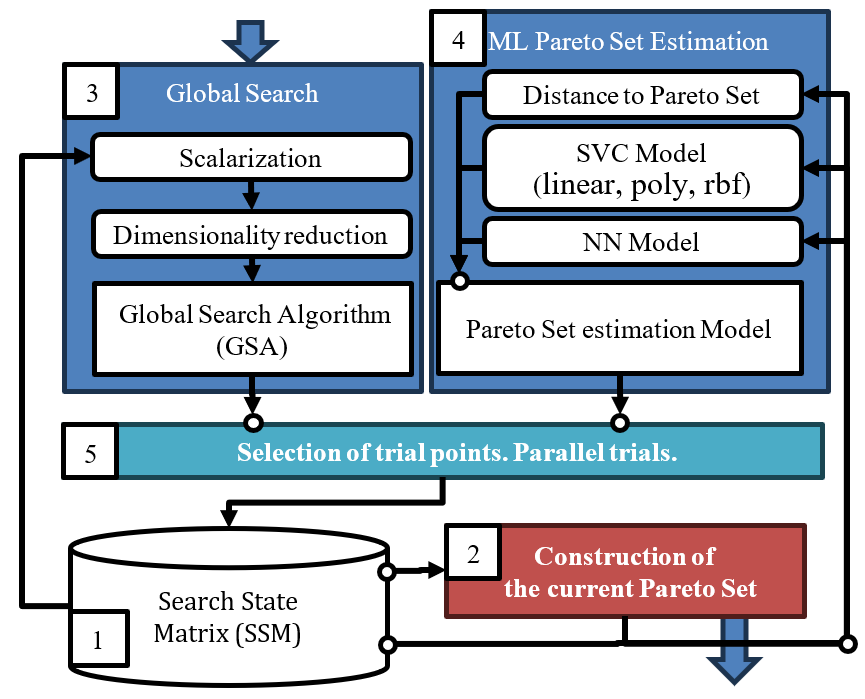
\includegraphics[width=0.7\textwidth]{fig1.png}
\caption{Computational scheme of the algorithm for solving multicriterial optimization problems using machine learning models.} \label{fig1}
\end{figure}


\subsection{Block of the global search algorithm}
\label{subsec31}

The search for a globally optimal solution to problem (\ref{eq:01})-(\ref{eq:03}) consists of the following basic steps:
\begin{enumerate}
	\item scalarization of efficiency criteria;
	\item dimensionality reduction;
	\item optimization on the base of the global search algorithm.
\end{enumerate}

\textbf{Scalarization of efficiency criteria.} It is possible to find the Pareto set either solving the problem in the original formulation \cite{Evtushenko2014,DPA02,Durillo2010,Mostaghim2007,Nebro2009,RC05,Zitzler2001}, or reducing the original problem to a series of scalar problems to find effective solutions \cite{Pardalos2017,Konnov2025,Gergel2019_2,Gergel2018,GergelKozinov2020}. 

In the framework of the developed approach \cite{Konnov2025}, the second option with scalarization of criteria is used. To build a good estimate of the Pareto set, a family of problems



\subsection{Block for accumulating and reusing the information about current state of the search}
\label{subsec32}

\subsection{Block for building the Pareto set estimation}
\label{subsec33}

\begin{figure}
\center
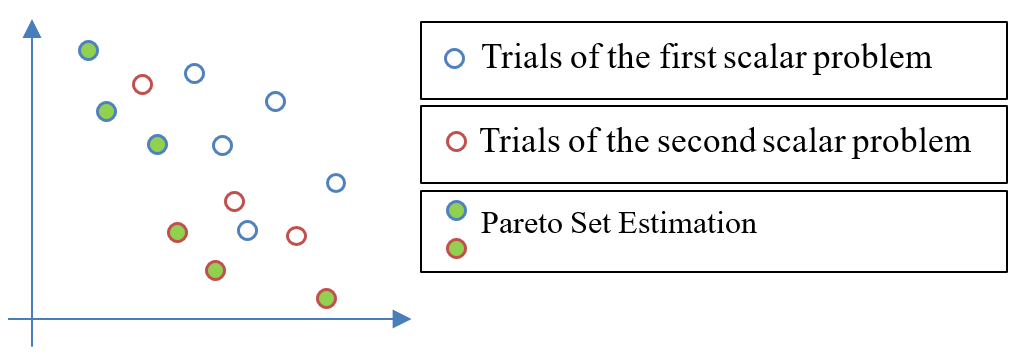
\includegraphics[width=0.6\textwidth]{fig2.png}
\caption{Example of Pareto set evaluation in solving two scalar optimization problems.} \label{fig2}
\end{figure}


\subsection{Block of  building the machine learning for estimation of the Pareto set}
\label{subsec34}

\begin{figure}
\center
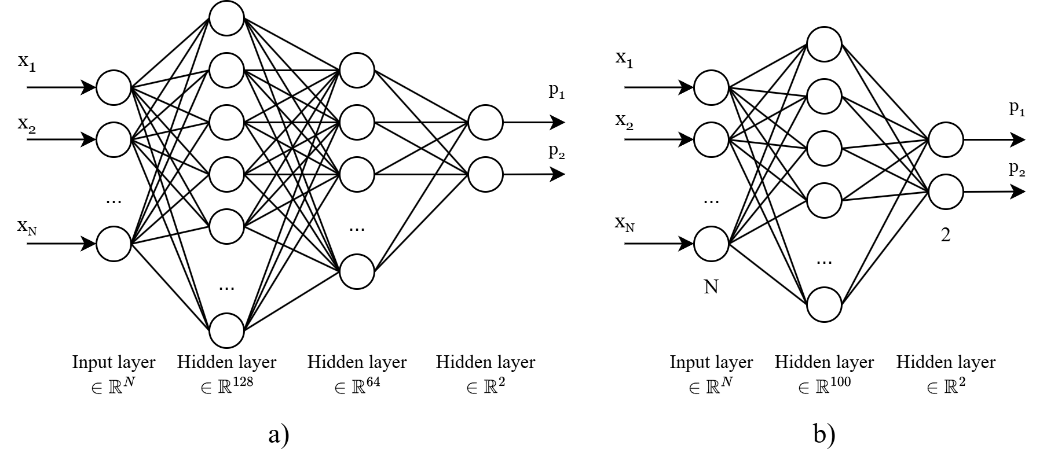
\includegraphics[width=0.8\textwidth]{fig3.png}
\caption{Neural network models used to calculate the characteristic $R_{PS}(i)$.} \label{fig3}
\end{figure}

\begin{figure}
\center
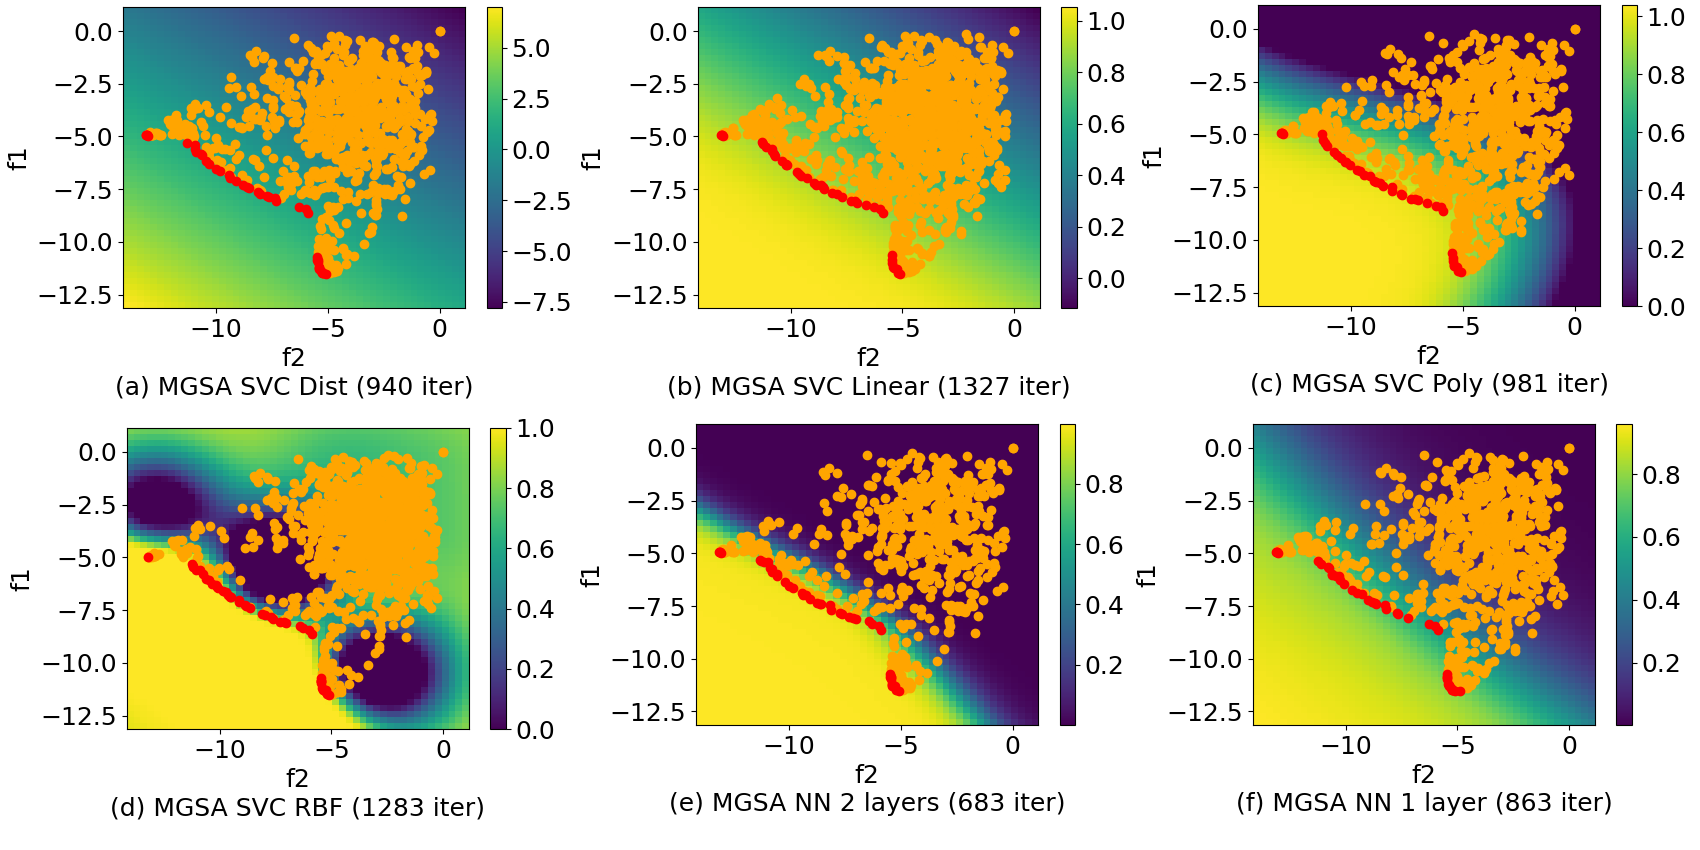
\includegraphics[width=0.6\textwidth]{fig4.png}
\caption{Examples of Pareto set evaluation for the case of two scalar optimization problems.} \label{fig4}
\end{figure}


\subsection{Block for the choice of trial points and implementation of computational experiments}
\label{subsec35}

\section{Results of computational experiments}
\label{sec4}

\begin{figure}
\center
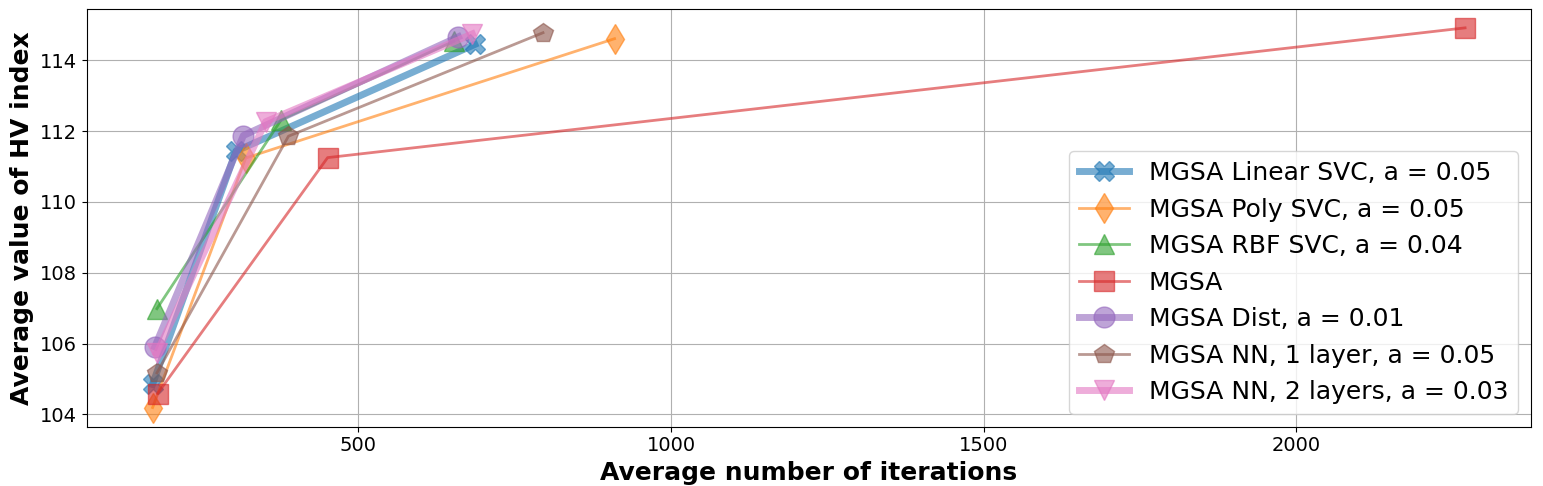
\includegraphics[width=0.8\textwidth]{fig5.png}
\caption{Comparison of HW index values for sequential algorithm implementation.} \label{fig5}
\end{figure}

% Please add the following required packages to your document preamble:
% \usepackage{graphicx}
\begin{table}[ht]
\centering
\caption{Average number of trials per process}
\label{tab:1}
\resizebox{0.8\textwidth}{!}{%
\begin{tabular}{ccccccc}
\hline
\textbf{Number of processes}            & \textbf{1}      & \textbf{2}      & \textbf{4}      & \textbf{8}      & \textbf{16}    & \textbf{20}    \\ \hline
MGSA                                    & 2269.82         & 1385.02         & 746.57          & 373.36          & 202            & 143.52         \\
\textbf{MGSA   Linear SVC,  a = 0.05}   & \textbf{686.13} & \textbf{408.79} & \textbf{213.6}  & \textbf{111.85} & \textbf{70.95} & \textbf{62.16} \\
MGSA   Poly SVC, a = 0.05               & 909.59          & 544.19          & 278.62          & 153.64          & 95.37          & 77.94          \\
MGSA   RBF SVC, a = 0.04                & 652.74          & 446.84          & 233.81          & 119.84          & 72.36          & 62.37          \\
\textbf{MGSA   Dist, a = 0.01}          & \textbf{659.98} & \textbf{402.9}  & \textbf{211.33} & \textbf{112.38} & \textbf{70.79} & \textbf{62.00} \\
MGSA   NN 1 layer, a = 0.05             & 795.16          & 446.25          & 232.08          & 117.16          & 75.19          & 62.70          \\
\textbf{MGSA   NN 2 layers, a =   0.03} & \textbf{682.12} & \textbf{401.74} & \textbf{219.62} & \textbf{113.32} & \textbf{73.51} & \textbf{61.32} \\ \hline
\end{tabular}%
}
\end{table}


\begin{table}[ht]
\centering
\caption{Average HW Index in dependence on number of processes}
\label{tab:2}
\resizebox{0.8\textwidth}{!}{%
\begin{tabular}{ccccccc}
\hline
Number of processes                   & \textbf{1}      & \textbf{2}      & \textbf{4}      & \textbf{8}      & \textbf{16}     & \textbf{20}     \\ \hline
\textbf{MGSA}                         & \textbf{114.91} & \textbf{114.79} & \textbf{114.84} & \textbf{114.90} & \textbf{115.00} & \textbf{114.96} \\
MGSA   Linear SVC, a = 0.05           & 114.44          & 114.65          & 114.72          & 114.74          & 114.91          & 114.96          \\
\textbf{MGSA   Poly SVC,    a = 0.05} & \textbf{114.61} & \textbf{114.64} & \textbf{114.71} & \textbf{114.8}  & \textbf{114.95} & \textbf{115.01} \\
MGSA   RBF SVC,    a = 0.04           & 114.54          & 114.54          & 114.73          & 114.89          & 114.92          & 114.96          \\
MGSA   Dist, a = 0.01                 & 114.66          & 114.55          & 114.69          & 114.73          & 114.92          & 114.93          \\
MGSA   NN 1 layer, a = 0.05           & 114.77          & 114.61          & 114.72          & 114.81          & 114.96          & 114.98          \\
\textbf{MGSA   NN 2 layers, a = 0.03} & \textbf{114.74} & \textbf{114.54} & \textbf{114.71} & \textbf{114.76} & \textbf{114.98} & \textbf{115.01} \\ \hline
\end{tabular}%
}
\end{table}

\begin{figure}
\center
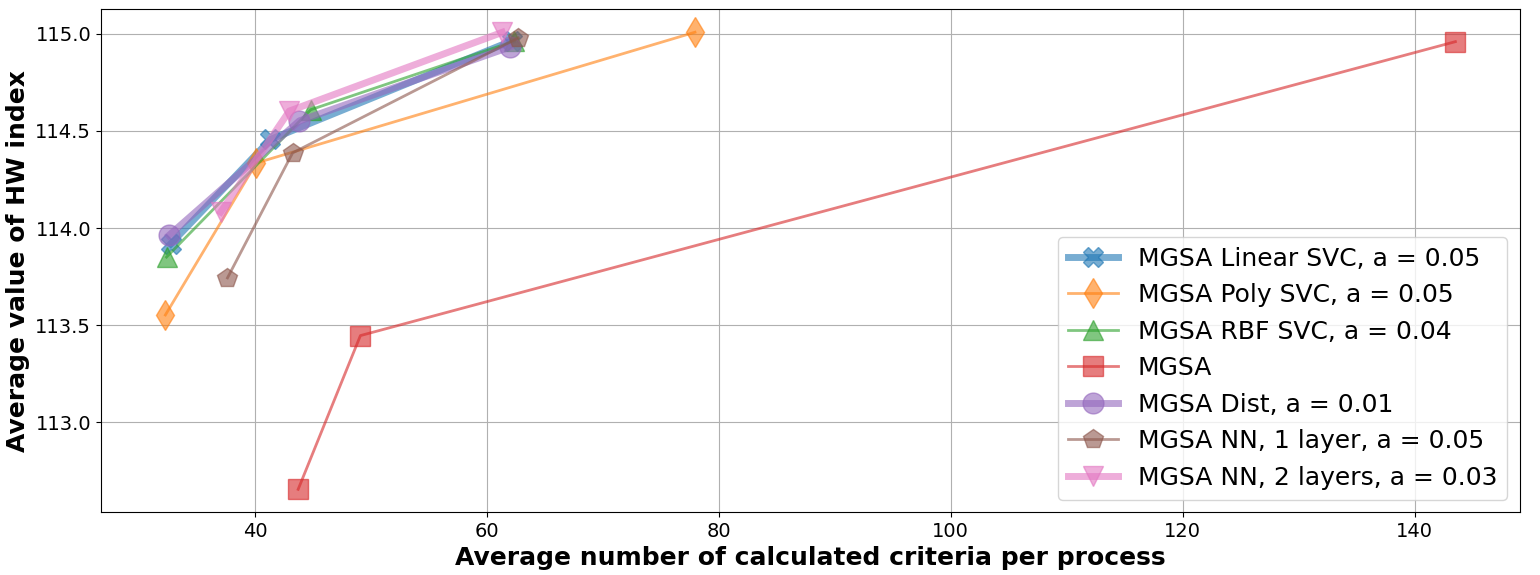
\includegraphics[width=0.8\textwidth]{fig6.png}
\caption{Dependence of the mean value of the index HW from the trial number per process for the case of 20 processes.} \label{fig6}
\end{figure}

\begin{figure}
\center
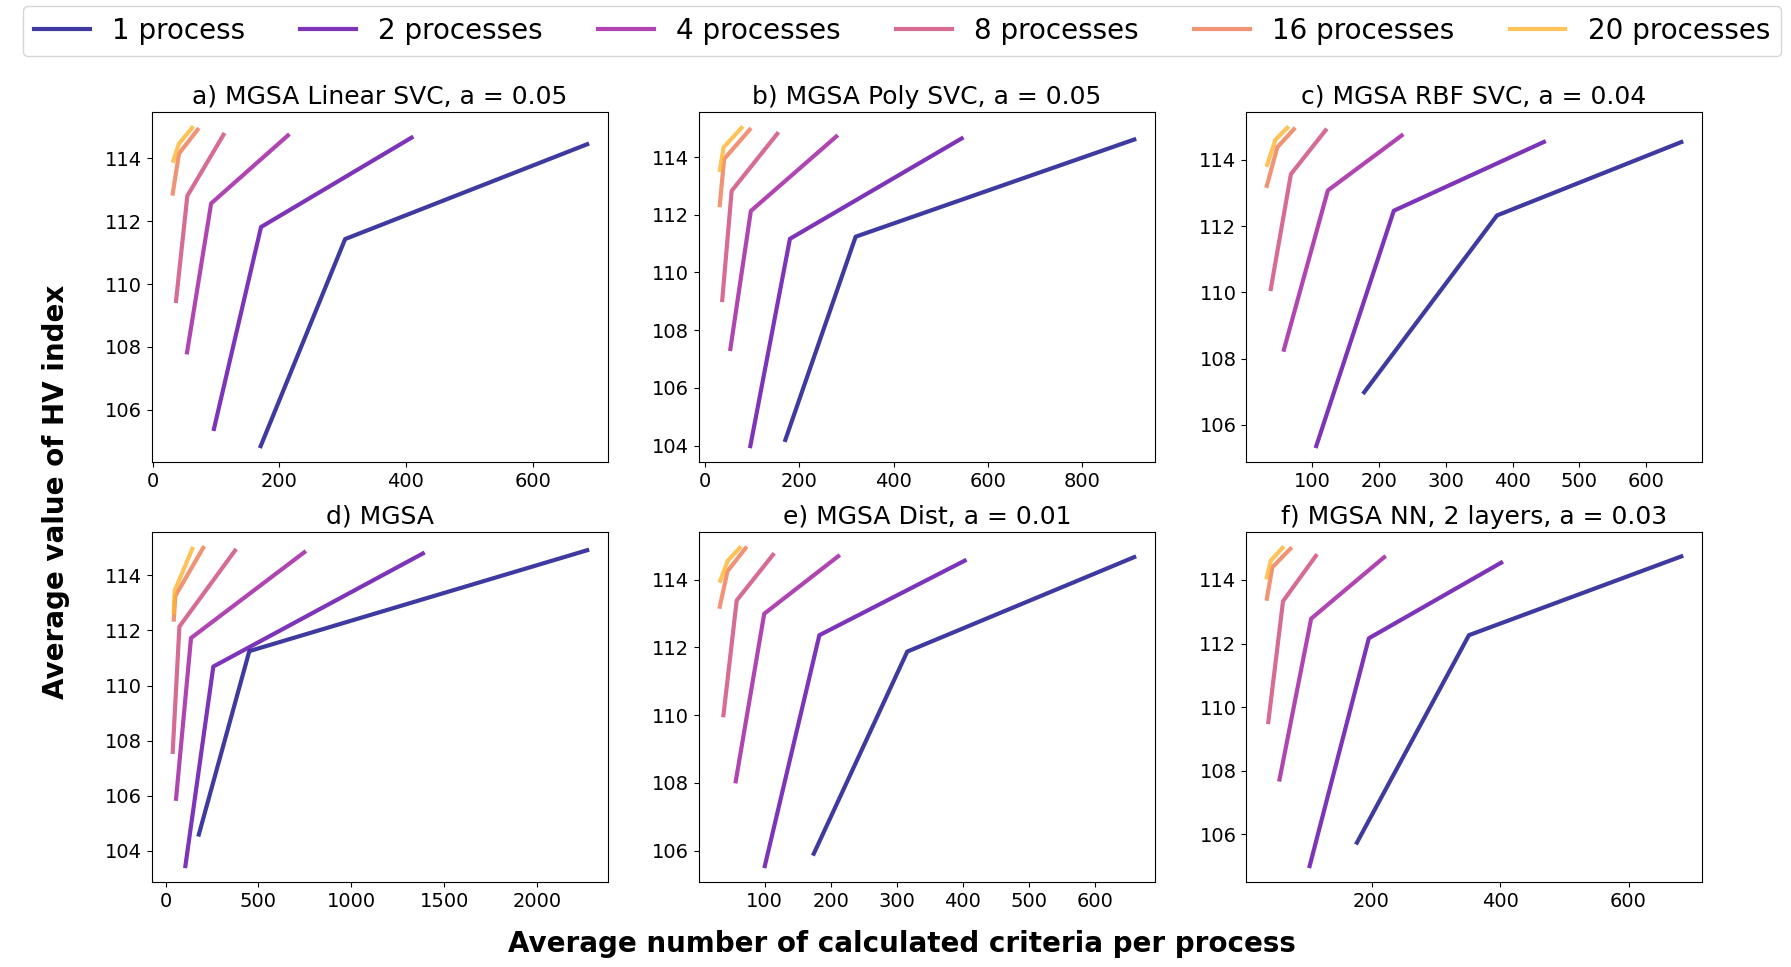
\includegraphics[width=0.8\textwidth]{fig7.png}
\caption{Dependence of the HW index on the number of trials executed for different number of processes.} \label{fig7}
\end{figure}


\section{Conclusion}
\label{sec5}
The research presents a parallel modification of the global search algorithm for solving multicriterial optimization problems. One of the features of the algo-rithm is the combination of the classic global search algorithm with machine learning methods. The combination of algorithms shows high efficiency in both sequential and parallel modifications. As the direction of further research it is planned to organize a number of experiments to solve applied problems and compare search efficiency with a number of third-party frameworks.


\begin{credits}
\subsubsection{\ackname} This study was funded by the ...

\subsubsection{\discintname}
The authors have no competing interests to declare that are relevant to the content of this article.
\end{credits}
%
% ---- Bibliography ----
%
% BibTeX users should specify bibliography style 'splncs04'.
% References will then be sorted and formatted in the correct style.
%
\bibliographystyle{splncs04}
\bibliography{bibliography}
%
%\begin{thebibliography}{8}
%\bibitem{ref_article1}
%Author, F.: Article title. Journal \textbf{2}(5), 99--110 (2016)
%
%\bibitem{ref_lncs1}
%Author, F., Author, S.: Title of a proceedings paper. In: Editor,
%F., Editor, S. (eds.) CONFERENCE 2016, LNCS, vol. 9999, pp. 1--13.
%Springer, Heidelberg (2016). \doi{10.10007/1234567890}
%
%\bibitem{ref_book1}
%Author, F., Author, S., Author, T.: Book title. 2nd edn. Publisher,
%Location (1999)
%
%\bibitem{ref_proc1}
%Author, A.-B.: Contribution title. In: 9th International Proceedings
%on Proceedings, pp. 1--2. Publisher, Location (2010)
%
%\bibitem{ref_url1}
%LNCS Homepage, \url{http://www.springer.com/lncs}, last accessed 2023/10/25
%\end{thebibliography}
\end{document}
